\documentclass[10pt,twoside]{article}

\usepackage{suppmat}
\usepackage{listings}
\usepackage[T1]{fontenc} % Better underscores, shockingly.

\newcommand{\plant}{\textsc{plant}}

\usepackage{graphicx}
% We will generate all images so they have a width \maxwidth. This means
% that they will get their normal width if they fit onto the page, but
% are scaled down if they would overflow the margins.
\makeatletter
\def\maxwidth{\ifdim\Gin@nat@width>\linewidth\linewidth\else\Gin@nat@width\fi}
\def\maxheight{\ifdim\Gin@nat@height>\textheight\textheight\else\Gin@nat@height\fi}
\makeatother
\setkeys{Gin}{width=\maxwidth,height=\maxheight,keepaspectratio}

\title{{\plant}: A package for modelling forest trait ecology \& evolution --
\emph{Description of the \texttt{FFW16} physiological model}}
\date{}

\usepackage[]{natbib}
\bibliographystyle{../mee}

\begin{document}

\maketitle

\tableofcontents

\section{Introduction}

The core job of the physiological model in {\plant} is to take a plant's
current size, light environment and physiological parameters as inputs,
and return it's growth, mortality and fecundity rates. In the default
physiological model within {\plant}, these vital demographic rates are all
derived from the rate at which living biomass is produced by the plant,
which in turn is calculated based on well understood physiology (Fig.
\ref{fig:schematic-phys}). Various physiological parameters
influence demographic outcomes. Varying these parameters allows for
species-differences to be included, potentially via traits (see last
section). Tables
\ref{tab:definitions}, \ref{tab:params_core},  \ref{tab:params_hyper} give
 units and definitions of all variables, parameters and hyper-parameters used in
 the material below.

\begin{figure}[h!]
\centering
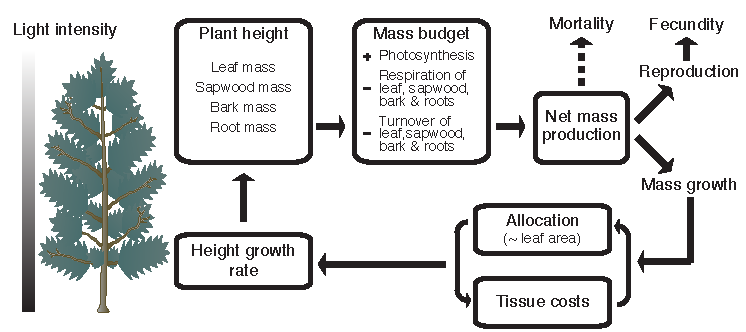
\includegraphics[width=15cm,height=15cm,keepaspectratio]{../figures/schematic-phys}
\caption{Physiological model in {\plant}, giving
demographic rates on the basis of its traits, size and light environment. as functions of
net mass production. The dashed line to mortality indicates that although mortality rate is assumed to depend on mass production, no
mass is actually allocated there.}
\label{fig:schematic-phys}
\end{figure}

\section{Leaf photosynthesis}\label{leaf-photosynthesis}

Let \(p(x, E)\) denote the gross rate of leaf photosynthesis per unit
area at height within the canopy of a plant with traits \(x\) at light
level \(E(z)\). We assume a relationship of the form
\begin{equation}\label{eq:photosynthesis}
p(x, E(z)) = \frac{\alpha_{p1}}{E(z) + \alpha_{p2}},
\end{equation}
for the average of \(p\) across the year. The parameters
\(\alpha_{p1}, \alpha_{p2}\) are derived from a detailed leaf-level
model and correspond to maximum annual photosynthesis and light-level
where photosynthesis is 50\% of it's maximum value. The average rate of
leaf photosynthesis across the plant is then
\begin{equation}\label{eq:photosynthesis_av}
\bar{p}(x, H, E_a) = \int_0^H p(x, E(z)) \, q(z, H),
\end{equation}
where \(q(z, H)\) gives the density of leaf area at height \(z\) (Eq.
\ref{eq:crown3}).

\section{Standard model for mass
production}\label{standard-model-for-mass-production}

The amount of biomass available for growth,
\(\rm{d}B / \rm{d}t\), is given by the difference between income
(total photosynthetic rate) and losses (respiration and turnover) within the
plant \citep{Makela-1997, Thornley-2000, Falster-2011}:
\begin{equation}\label{eq:dbdt}
\underbrace{\strut \frac{\rm{d}B}{\rm{d}t}}_\textrm{net biomass production}
  = \underbrace{\strut a_y}_\textrm{yield}
    \big( \underbrace{\strut A_\textrm{l} \, \bar{p}}_\textrm{photosynthesis} -
     \underbrace{\strut \, \sum_\textrm{i = l, b, s, r}{M_\textrm{i} \, r_\textrm{i}}}_\textrm{respiration}\big)
    - \underbrace{\strut \sum_\textrm{i = l, b, s, r}{M_\textrm{i} \, k_\textrm{i}}}_\textrm{turnover}.
\end{equation}
Here, \(M, r\), and \(k\) refer to the mass, maintenance respiration rate, and
turnover rate of different tissues, denoted by subscripts \(l\) = leaves,
\(b\) = bark, \(s\) = sapwood and \(r\) = roots. \(\bar{p}\) is the assimilation
rate of CO\(_2\) per leaf area and \(y\) is yield: the fraction of
assimilated carbon fixed in biomass (the remaining fraction being lost
as growth respiration). The growth respiration component comes in addition
to any costs of maintenance respiration. Gross photosynthetic production is proportional to leaf area,
\(A_\textrm{l} = M_\textrm{l} / \phi\), where \(\phi\) is leaf mass per
area. The total mass of living tissues
\(M_\textrm{a} = M_\textrm{l} + M_\textrm{b} + M_\textrm{s} + M_\textrm{r}.\)

\section{Height growth rate}\label{height-growth-rate}

The key measure of growth required by the demographic solver is
rate of height growth for the plant, $g(x, H, E_a)$. To model growth in
height requires that we translate mass
production into height increment, accounting for the costs of
building new tissues, allocation
to reproduction, and architectural layout. Mathematically, height growth
can be decomposed into a product of physiologically relevant terms
\citep{Falster-2011}:
\begin{equation} \label{eq:dhdt}
g(x, H, E_a) = \frac{\rm{d}H}{\rm{d}t} = \frac{\rm{d}H}{\rm{d}A_\textrm{l}}
\times \frac{\rm{d}A_\textrm{l}}{\rm{d}M_\textrm{a}}
\times \frac{\rm{d}M_\textrm{a}}{\rm{d}B}
\times \frac{\rm{d}B}{\rm{d}t}.
\end{equation}

The first term on the right of eq \ref{eq:dhdt},
\(\rm{d}H / \rm{d}A_\textrm{l}\), is the growth in plant height
per unit growth in total leaf area -- accounting for the architectural
strategy of the plant. Some species tend to leaf out more than grow
tall, while other species emphasise vertical extension.

The second term in eq \ref{eq:dhdt},
\(\rm{d}A_\textrm{l} / \rm{d}M_\textrm{a}\), accounts for the
marginal cost of deploying an additional unit of leaf area, including
construction of the leaf itself and various support structures. As such,
\(\rm{d}A_\textrm{l} / \rm{d}M_\textrm{a}\) can itself be
expressed as a sum of construction costs per unit leaf area:
\begin{equation}\label{eq:daldmt}
\frac{\rm{d}A_\textrm{l}}{\rm{d}M_\textrm{a}}
= \big( \frac{\rm{d}M_\textrm{l}}{\rm{d}A_\textrm{l}} + \frac{\rm{d}M_\textrm{s}}{\rm{d}A_\textrm{l}} + \frac{\rm{d}M_\textrm{b}}{\rm{d}A_\textrm{l}} + \frac{\rm{d}M_\textrm{r}}{\rm{d}A_\textrm{l}}\big)^{-1}.
\end{equation}

The third term in eq \ref{eq:dhdt},
\(\rm{d}M_\textrm{a} / \rm{d}M_\textrm{b}\), gives the fraction
of net biomass production (eq. \ref{eq:dbdt}) that is allocated to
growth rather than reproduction or storage. In the default physiological model
we let the growth fraction decrease with height according to the function
\begin{equation}\label{eq:allocation}
\frac{\rm{d}M_\textrm{a}}{\rm{d}B}(H) = 1 -
 \frac{\alpha_{r1}} {1.0 + \exp\left(\alpha_{r2}  \left(1.0 - H / H_{mat}\right)\right)},
\end{equation}
where $\alpha_{r1}$ is the maximum possible allocation (0-1) and $\alpha_{r2}$
determines the sharpness of the transition.

\section{Diameter growth rate}

In a similar way, basal area ($A_\textrm{st}$) increment can be
expressed as the sum of increments in sapwood, bark \& heartwood areas
($A_\textrm{s}, A_\textrm{b}, A_\textrm{H}$ respectively):
$$\frac{\rm{d}A_\textrm{st}}{\rm{d}t} = \frac{\rm{d}A_\textrm{b}}{\rm{d}t} + \frac{\rm{d}A_\textrm{s}}{\rm{d}t} + \frac{\rm{d}A_\textrm{H}}{\rm{d}t}.$$
We now have an equation for basal area growth that contains many of the same
elements as eq. \ref{eq:dhdt}:
\begin{equation}\label{eq:dast}
\frac{\rm{d}A_\textrm{st}}{\rm{d}t} = \left(\frac{\rm{d}A_\textrm{s}}{\rm{d}A_\textrm{l}} + \frac{\rm{d}A_\textrm{b}}{\rm{d}A_\textrm{l}}\right) \times
\frac{\rm{d}A_\textrm{l}}{\rm{d}M_\textrm{a}} \times \frac{\rm{d}M_\textrm{a}}{\rm{d}B} \times \frac{\rm{d}B}{\rm{d}t} + \frac{\rm{d}A_\textrm{H}}{\rm{d}t} .
\end{equation}
Diameter growth is then given by the geometric relationship between stem
diameter ($D$) and $A_\textrm{st}$:
\begin{equation} \label{eq:dDdt}
\frac{\rm{d}D}{\rm{d}t} = \sqrt{\frac{\pi}{A_\textrm{st}}} \frac{\rm{d}A_\textrm{st}}{\rm{d}t}.
\end{equation}

\section{A functional-balance model for
allocation}\label{a-functional-balance-model-for-allocation}

Here we describe an allometric model linking the various size dimensions
of a plant required by most ecologically realistic vegetation models
(i.e. = mass of leaves, mass of sapwood, mass of bark, mass of fine
roots) to a plant's height. This approach allows us to track only the
plant's height, while still accounting for the mass need to build
leaves, roots, and stems. The growth rates of various tissues can then
also be derived (Table \ref{tab:allometry}).

\subsection{Leaf area}\label{leaf-area}

Based on empirically observed allometry, we assume an allometric log-log
scaling relationship between the accumulated leaf area of a plant and
its height:
\begin{equation}\label{eq:ha}
A_\textrm{l} = \alpha_{l1} \, H^{\alpha_{l2}}.
\end{equation}
Note, scaling relationship reversed from \citep{Falster-2011}.

\subsection{Vertical distribution of leaf
area}\label{vertical-distribution-of-leaf-area}

We follow the model of \citet{Yokozawa-1995} describing the vertical
distribution of leaf area within the crowns of individual plants. This
model can account for a variety of canopy profiles through a single
parameter \(\eta\). Setting \(\eta = 1\) results in a conical canopy, as
seen in many conifers, while higher values, e.g. \(\eta = 12\) , gives a
top-weighted canopy profile similar to those seen among angiosperms. Let
\(A_\textrm{s}(z)\) be the sapwood area at height \(z\) for a plant with
top height \(H\), \(A_\textrm{s}\) ($= A_\textrm{s}(0)$) be the sapwood
area at the base of the plant, \(q(z, H)\) the probability density of
leaf area at height \(z\) and \(Q(z, H)\) the cumulative fraction of a
plant's leaf above height \(z\). Following \citet{Yokozawa-1995} we
assume a relationship between \(A_\textrm{s}(z)\) and height such that
\begin{equation}\label{eq:crown1}
\frac{A_\textrm{s}(z)}{A_\textrm{s}} = \left(1 - \left(\frac{z}{H}\right)^\eta\right)^2.
\end{equation}

We also assume that each unit of sapwood area supports a fixed area of
leaf \citep[the pipe model][]{Shinozaki-1964}, so that the total canopy
area of a plant relates to basal sapwood area \(A_\textrm{s}\):
\begin{equation}\label{eq:crown2}
\frac{M_\textrm{l}}{\phi} = \theta \, A_\textrm{s}.
\end{equation}
The pipe model is assumed to hold within individual plants, as well as
across plants of different size. It then follows that
\begin{equation}\label{eq:crown1}
Q(z, H) = \left(1-\left(\frac{z}{H}\right)^\eta\right)^2.
\end{equation}
Differentiating with respect to \(z\) then yields a solution for the
probability density of leaf area as a function of height:
\begin{equation}\label{eq:crown3}
q(z, H) = 2\frac{\eta}{H}\left(1-\left(\frac{z}{H}\right)^{\eta}\right) \left(\frac{z}{H}\right)^{\eta-1}.
\end{equation}

\subsection{Mass of sapwood}\label{mass-of-sapwood}

Integrating \(A_\textrm{s}(z)\) gives a solution for the total mass of
sapwood in the plant:
\begin{equation}\label{eq:ms1}
M_\textrm{s} = \rho \, \int_0^h \, A_\textrm{s}(z) \, \rm{d}z = \rho \, A_\textrm{s} \, H \, \eta_c,
\end{equation}
where \(\eta_c = 1 - \frac{2}{1 + \eta} + \frac{1}{1 + 2\eta}\)
\citep{Yokozawa-1995}. Substituting from Eq. \ref{eq:crown2} into Eq.
\ref{eq:ms1} then gives an expression for sapwood mass as a function
leaf area and height:
\begin{equation}\label{eq:ms2}
M_\textrm{s} = \rho \, \eta_c \, \theta \, A_\textrm{l} \, H.
\end{equation}

\subsection{Bark mass}\label{bark-mass}

Bark and phloem tissue are modelled using an analogue of the pipe model,
leading to a similar equation as that for sapwood mass (Eq.
\ref{eq:ms2}). Cross sectional-area of bark per unit leaf area is
assumed to be a constant fraction \(b\) of sapwood area per unit leaf
area such that
\begin{equation}\label{eq:mb}
M_\textrm{b} = \alpha_{b1} M_\textrm{s}.
\end{equation}

\subsection{Root mass}\label{root-mass}

Also consistent with pipe-model assumption, we assume a fixed ratio of
root mass per unit leaf area
\begin{equation}\label{eq:mr}
M_\textrm{r} = \alpha_{r1} \, A_\textrm{l}.
\end{equation}
Even though nitrogen and water uptake are not modelled explicitly,
imposing a fixed ratio of root mass to leaf area ensures that
approximate costs of root production are included in calculations of
carbon budget.

\section{Seed production}\label{seed-production}

The rate of seed production from the plant \(f(x, H, E_a)\) is a direct
function of mass allocated to reproduction:
\begin{equation}\label{eq:fecundity}
f(x, H, E_a) = \frac{(1 - \frac{\rm{d}M_\textrm{a}}{\rm{d}B}) \times \frac{\rm{d}B}{\rm{d}t}}{
  s + \alpha_{f3}},
\end{equation}
where \(s\) is the mass of the seed and \(\alpha_{f3}\) is the cost
per seed of accessories, such as fruits, flowers and dispersal
structures. The function $\frac{\rm{d}M_\textrm{a}}{\rm{d}B}$ gives the fraction
of $\frac{\rm{d}B}{\rm{d}t}$ that is allocated to growth, while
$1-\frac{\rm{d}M_\textrm{a}}{\rm{d}B}$ gives the  fraction allocated
to reproduction.

\section{Mortality}\label{mortality}

Instantaneous rates of plant mortality are taken as the sum of a growth
independent and growth dependent terms
\citep{Falster-2011, Moorcroft-2001}:
\begin{equation}\label{eq:mortality}
d(x, H, E_a) = d_{\textrm{I}}(x, H) + d_{\textrm{D}}(x, H, E_a).
\end{equation}
The growth independent rate is taken to be a constant, independent of
plant performance, but potentially varying with species traits. The
growth dependent part is assumed to decline exponentially with the rate
of mass production per unit leaf area, i.e.
\begin{equation}\label{eq:mortality_GD}
d_{\textrm{D}}(x, H, E_a) = \alpha_{d2}  \exp(-\alpha_{d3} X),
\end{equation}
where \(X = \rm{d}B / \rm{d}t / A_\textrm{l}\). This
relationship allows for plants to increase mortality as growth rate
approaches zero, while also allowing for differences among species in
the parameters \(\alpha_{d2}\) and \(\alpha_{d3}\).

We also require a function \(S_G(x^\prime, H_0, E_{A_0})\) for survival
through germination. For the demographic model to behave smoothly,
\(S_G (x^\prime, H_0, E_{A_0}) / g(x, H_0, E_{A_0})\) should approach zero as
\(g(x, H_0, E_{A_0}) \rightarrow 0\). Following \citep{Falster-2011},
we use the function
\begin{equation} \label{eq:pi1}
  S_G (x^\prime, H_0, E_{A_0}) = \frac1{X^2 + 1.0}
\end{equation}
where $X = \alpha_{d0} \frac{A_l}{\rm{d}B / \rm{d}t}$ and $\alpha_{d0}$ is a
constant. The behaviour of Eq. \ref{eq:pi1} is consistent with Eq.
\ref{eq:mortality_GD}, as both cause survival to decline with mass production.

\section{Hyper-parameterisation of physiological model via
traits}\label{traits}

The plant physiological model includes default values for all parameters needed
(see Table \ref{tab:params_core}). Species are known to vary considerably
in many of these parameters, such as $\phi,\rho, \alpha_{p1}, s$; so by varying  parameters
one can account for different ecologies. When altering one parameter in the model, however,
one must also consider whether there are trade-offs linking parameters.

{\plant} allows for
hyper-parameterisation of the plant physiological model via plant functional traits, i.e.
simultaneous variation in multiple parameters because of assumed trade-off. In the
default physiological model we implement the following relationships. For more
details see \texttt{make\_FFW16\_hyperpar.R}.

\subsection{Leaf mass per area}

The trait leaf mass per area ($\phi$) directly influences growth by changing
$\rm{d}A_\textrm{l} / \rm{d}M_\textrm{a}$. In addition we
link $\phi$ to the rate of leaf turnover,
based on widely observed scaling relationship from \citet{Wright-2004}:
$$k_l = \beta_{kl1} \, \left(\frac{\phi}{\phi_0}\right)^{-\beta_{kl2}}.$$
We normalise the relationship around a global mean \textsc{lma} of $\phi_0$ -- this
allows us to vary $\beta_{kl1}$ and $\beta_{kl2}$ without displacing the relationship from the
observed mean.
We also vary mass based leaf respiration rate so that it stays constant per unit leaf area and
varies with \textsc{lma}, as is empirically observed \citet{Wright-2004}:
$$r_\textrm{l} = \frac{c_{Rl0}}{\phi}.$$

\subsection{Wood density}

The trait wood density ($\rho$) directly influences growth by changing
$\rm{d}A_\textrm{l} / \rm{d}M_\textrm{a}$.  In addition we
link $\rho$ to the rate of growth independent mortality:
$$d_I = \beta_{dI1} \, \left(\frac{\rho}{\rho_0}\right) ^ {-\beta_{dI2}}.$$
In addition, $\rho$ is assumed to influence the rate of sapwood turnover,
$$k_s = \beta_{ks1} \, \left(\frac{\rho}{\rho_0}\right)^ {-\beta_{ks2}},$$
and the rate of sapwood respiration per unit mass:
$$r_r = \frac{4012.0}{\rho}.$$
As with $\phi$, we normalise the mortality and turnover
relationships around a global mean value of $\rho_0$.

\subsection{Seed mass}

Effects of the trait seed mass ($s$) are naturally embedded in the equation determining
fecundity (Eq. \ref{eq:fecundity}) and the initial height of seedlings (XXX). In addition,
we let the accessory cost per seed be a linear function of seed size:
$$\alpha_{f3} = 3.0 * s,$$
following observed relationships \citep{Henery-2001}.

\subsection{Nitrogen per leaf area}

Photosynthesis per unit leaf area and respiration rates per unit leaf mass (or area)
are assumed to vary with leaf nitrogen per unit area $\nu$:
$$\alpha_{p1} = c_{PN} \, \nu,$$
$$r_l = c_{RN} \, \nu.$$

\clearpage

\section{Tables}\label{tables}

\begin{table}[h!]
 \caption{Key variables in physiological model.
 Subscripts $i = l, s, b, r, a$ refer to leaves, sapwood, roots, total of these vegetative tissues. Similarly $A_i$ denotes areas, of leaves ($i = l$) and of cross-sections of total stem and sapwood ($i = st, ss$) respectively.}
\centering
  \begin{tabular}{p{2cm}p{2cm}p{8cm}}
  \hline
  Symbol & Unit & Description \\
  \hline
  $H$   & m  & height of plant\\
  $B$   & kg  & biomass originating from parent plant\\
  $M_i$ & kg  & mass retained on plant in tissue $i$\\
  $A_i$ & m$^2$  & surface-area or cross-sectional-area of tissue $i$\\
  $y$ & kg kg$^{-1}$ & Yield; ratio of carbon fixed in mass per carbon assimilated \\
  $p,\bar{p}$ & kg yr$^{-1}$ m$^{-2}$  & photosynthetic rate per unit area \\
  $r_i$ & kg yr$^{-1}$ kg$^{-1}$  & respiration per unit tissue mass \\
  $k_i$ & yr$^{-1}$ & turnover rate for tissue \\
  \hline
  \end{tabular}
\label{tab:definitions}
\end{table}

\newpage

\begin{table}[h!]
\caption{Equations for an allometric growth model, based on functional balance assumptions.
The key assumptions of the physiological model are listed in a), under "function". From these
assumptions we derive allocation functions for both tissue areas and masses (b). We can also
express growth rate for each tissue as a function of growth rate in leaf area. }
\centering
  \begin{tabular}{p{2.5cm}p{3.5cm}p{5cm}p{4cm} }\\ \hline
  Variable & Function & Allocation & Growth rate\\ \hline
  \multicolumn{4}{l}{\textbf{a) Assumed relationship to leaf area}} \\ \\
  height &
    $H = \alpha_{l1} \, A_\textrm{l}^{\alpha_{l2}}$ &
    $\frac{\rm{d}H}{\rm{d}A_\textrm{l}} = \alpha_{l2} \alpha_{l1} A_\textrm{l}^{\alpha_{l2}-1}$ &
    $\frac{\rm{d}H}{\rm{d}t} = \frac{\rm{d}H}{\rm{d}A_\textrm{l}} \, \frac{\rm{d}A_\textrm{l}}{\rm{d}t}$ \\
  sapwoood area &
    $A_\textrm{s} = \theta \, A_\textrm{l}$ &
    $\frac{\rm{d}A_\textrm{s}}{\rm{d} A_\textrm{l}} = \theta$ &
    $\frac{\rm{d}A_\textrm{s}}{\rm{d}t} = \frac{\rm{d}A_\textrm{s}}{\rm{d} A_\textrm{l}} \, \frac{\rm{d}A_\textrm{l}}{\rm{d}t}$ \\
  bark area &
    $A_\textrm{b} = \alpha_{b1} \, \theta \, A_\textrm{l}$ &
    $\frac{\rm{d}A_\textrm{b}}{\rm{d} A_\textrm{l}} = \alpha_{b1} \, \theta$ &
    $\frac{\rm{d}A_\textrm{b}}{\rm{d}t} = \frac{\rm{d}A_\textrm{b}}{\rm{d} A_\textrm{l}} \, \frac{\rm{d}A_\textrm{l}}{\rm{d}t}$ \\  \\
  \multicolumn{4}{l}{\textbf{b) Derived equation for mass of tissue }} \\
  leaf mass &
    $M_\textrm{l} = \phi \, A_\textrm{l} $ &
    $\frac{\rm{d}M_\textrm{l}}{\rm{d}A_\textrm{l}} = \phi$ &
    $\frac{\rm{d}M_\textrm{l}}{\rm{d}t} = \frac{\rm{d}M_\textrm{l}}{\rm{d}A_\textrm{l}} \, \frac{\rm{d}A_\textrm{l}}{\rm{d}t}$ \\
  sapwood mass &
    $M_\textrm{s} = \theta \, \rho \, \eta_c \, A_\textrm{l} \, H $ &
    $\frac{\rm{d}M_\textrm{s}}{\rm{d}A_\textrm{l}} = \theta \, \rho \, \eta_c \, \big(H + A_\textrm{l} \, \frac{\rm{d}H}{\rm{d}A_\textrm{l}} \big)$ &
    $\frac{\rm{d}M_\textrm{s}}{\rm{d}t} = \frac{\rm{d}M_\textrm{s}}{\rm{d}A_\textrm{l}} \, \frac{\rm{d}A_\textrm{l}}{\rm{d}t}$ \\
  bark mass &
    $M_\textrm{b} = \alpha_{b1} \, \theta \, \rho \, \eta_c \, A_\textrm{l} \, H $ &
    $\frac{\rm{d}M_\textrm{b}}{\rm{d}A_\textrm{l}} = \alpha_{b1} \, \theta \, \rho \, \eta_c\big(H + A_\textrm{l} \, \frac{\rm{d}H}{\rm{d}A_\textrm{l}} \big)$ &
    $\frac{\rm{d}M_\textrm{b}}{\rm{d}t} = \frac{\rm{d}M_\textrm{b}}{\rm{d}A_\textrm{l}} \, \frac{\rm{d}A_\textrm{l}}{\rm{d}t}$ \\
  root mass &
    $M_\textrm{r} = \alpha_{r1} \, A_\textrm{l}$ &
    $\frac{\rm{d}M_\textrm{r}}{\rm{d}A_\textrm{l}} = \alpha_{r1}$  &
    $\frac{\rm{d}M_\textrm{r}}{\rm{d}t} = \frac{\rm{d}M_\textrm{r}}{\rm{d}A_\textrm{l}} \, \frac{\rm{d}A_\textrm{l}}{\rm{d}t}$ \\
  \hline \\
\end{tabular}
\label{tab:allometry}
\end{table}

\newpage

\begin{table}[h!]
\caption{Core model parameters}
\input{growth_model_pars_core}
\label{tab:params_core}
\end{table}

\begin{table}[h!]
\caption{Parameters for hyper-parameterisation}
\input{growth_model_pars_hyper}
\label{tab:params_hyper}
\end{table}

\clearpage

\bibliography{../refs}


\end{document}
